% Basic LaTeX template
\documentclass[11pt]{article}

% Page layout
\usepackage[margin=1in]{geometry}

% Common packages
\usepackage{graphicx}
\usepackage{float}
\usepackage{booktabs}
\usepackage[font=small,labelfont=bf]{caption}
\usepackage{amsmath,amssymb}
\usepackage{siunitx}
\usepackage[hidelinks]{hyperref}

% Metadata
\title{Aerodynamic and Structural Analysis of the Clipper Liberty C96 Wind Turbine}
\author{Evan Hobday, Peyton Lettau, Jordan Nguyen}
\date{\today}

\begin{document}

\maketitle

\begin{center}
\begin{minipage}{0.9\textwidth}
\small\textit{AI Assistance Disclosure: Artificial intelligence was used to help troubleshoot bugs in the code, provide justifications and reasoning behind the results, assist with formatting and organizing this report, and to format code blocks and plots generated by the code.}
\end{minipage}
\end{center}

\begin{abstract}
This report presents a comprehensive aerodynamic and structural analysis of the University of Minnesota's Clipper Liberty C96 wind turbine located in Rosemount, MN. The analysis employs Blade Element Momentum (BEM) theory to evaluate aerodynamic performance through coefficient of power ($C_P$) and thrust ($C_T$) calculations, pitch optimization, and two-dimensional parameter sweeps. Structural assessment focuses on tower deflection analysis, static failure evaluation using multiple failure theories, and fatigue analysis via Goodman criteria. Key findings include a maximum $C_P$ of 0.4464 at optimal pitch conditions, tower deflection of 0.383 meters (0.25\% of tower height), and safety factors of 8.11 for static failure and 3.418 for fatigue failure. The analysis reveals model limitations under extreme operating conditions where $C_P$ values exceed physical limits. All safety factors exceed the recommended minimum of 2.0, indicating adequate structural integrity under the analyzed loading conditions.
\end{abstract}

\begin{figure}[H]
  \centering
  \includegraphics[width=0.7\textwidth]{media/UMN\space Turbine.jpg}
  \caption{The University of Minnesota Clipper Liberty C96 wind turbine}
  \label{fig:umn_turbine_photo}
\end{figure}

\tableofcontents
\newpage

\section{Introduction}

Modern utility-scale wind turbines represent a critical component of renewable energy infrastructure, converting atmospheric kinetic energy into electricity through aerodynamic blade systems that drive generators via rotating shafts. As wind energy capacity continues to expand globally, understanding both the aerodynamic performance and structural integrity of these systems becomes increasingly important for optimal design and safe operation.

This report presents a comprehensive analysis of the University of Minnesota's Clipper Liberty C96 wind turbine located in Rosemount, MN. The study addresses two primary objectives: (1) quantifying aerodynamic performance through detailed analysis of power and thrust coefficients, and (2) assessing structural integrity under representative operating conditions to ensure safe and reliable operation.

\subsection{Analysis Approach}

The aerodynamic analysis employs Blade Element Momentum (BEM) theory, a well-established method for wind turbine performance prediction that combines momentum theory with blade element theory. This approach enables computation of thrust and power characteristics, evaluation of coefficients of power ($C_P$) and thrust ($C_T$), and exploration of optimal operating conditions through pitch optimization and two-dimensional parameter sweeps.

The structural assessment focuses on three key aspects: (1) tower deflection analysis under distributed wind loading and concentrated nacelle thrust, (2) static failure evaluation using Maximum Normal Stress, Maximum Shear Stress, and Distortion Energy, and (3) fatigue analysis employing modified Goodman criteria to assess long-term structural integrity.

\subsection{Implementation and Assumptions}

The complete analysis workflow is implemented in MATLAB using provided turbine specifications and material properties. Key assumptions include steady-state operating conditions, linear-elastic material behavior, no aerodynamic interference between blades, a pure bending stress state, and a rigid nacelle region. These assumptions enable manageable analytical solutions while maintaining sufficient accuracy for engineering design purposes.

\section{Methods}

This section presents the theoretical framework and computational methodology employed to analyze both the aerodynamic performance and structural integrity of the Clipper Liberty C96 wind turbine. The analysis is divided into two main components: aerodynamic analysis using Blade Element Momentum (BEM) theory and structural analysis employing beam theory and failure criteria.


\subsection{Aerodynamic Analysis}

The aerodynamic analysis employs Blade Element Momentum (BEM) theory to determine the performance characteristics of the wind turbine under various operating conditions. This section presents the methodology for calculating coefficients of power and thrust, followed by optimization procedures for determining optimal operating parameters.

\subsubsection{Fundamental BEM Theory}

The analysis begins with the calculation of fundamental aerodynamic parameters. For a given wind speed $V_\infty$, rotational speed $n$ (in RPM), and pitch angle $\beta$, the tip-speed ratio and angular velocity are calculated as:
\begin{equation}
\lambda = \frac{\omega R}{V_\infty}, \qquad \omega = \frac{2\pi n}{60}
\label{eq:tsr_omega}
\end{equation}
where $\lambda$ is the tip-speed ratio, $\omega$ is rotor speed [rad/s], $R$ is rotor radius, $n$ is rotor speed [RPM], and $V_\infty$ is the freestream wind speed.

\subsubsection{Induction Factors and Flow Angles}

The BEM theory requires the determination of axial and tangential induction factors. For the initial analysis, the axial induction factor is set to $a = 1/3$, which represents the momentum limit for maximum power extraction. The local tip-speed ratio at any radial position $r$ is calculated as:
\begin{equation}
\lambda_r = \lambda\, \frac{r}{R}
\label{eq:lambda_r}
\end{equation}
The tangential induction factor $a'$ is then calculated using the momentum balance:
\begin{equation}
a' = -\tfrac{1}{2} + \tfrac{1}{2}\, \sqrt{\,1 + \tfrac{4}{\lambda_r^{2}}\, a(1-a)\,}\, .
\label{eq:aprime}
\end{equation}
The inflow angle $\phi$, which represents the angle between the rotor plane and the relative wind velocity, is determined by:
\begin{equation}
\phi = \tan^{-1}\!\left( \frac{1 - a}{(1 + a')\,\lambda_r} \right)
\label{eq:phi}
\end{equation}
The local angle of attack $\alpha$ is then calculated by subtracting the geometric twist angle $\theta$ and pitch angle $\beta$ from the inflow angle:
\begin{equation}
\alpha = \phi - (\theta + \beta)
\label{eq:alpha}
\end{equation}
where $\theta$ is the local geometric twist and $\beta$ is the blade pitch angle.
\subsubsection{Airfoil Performance and Force Calculations}

Once the angle of attack is determined, the coefficients of lift ($C_L$) and drag ($C_D$) are obtained through interpolation of airfoil performance data. For circular sections (such as the blade root), the drag coefficient is calculated using a provided function for circular cylinders in cross-flow.

The lift and drag coefficients are then resolved into normal and tangential force coefficients relative to the rotor plane:
\begin{equation}
 C_n = C_L\cos\phi + C_D\sin\phi, \qquad C_t = C_L\sin\phi - C_D\cos\phi
\label{eq:cn_ct}
\end{equation}

\subsubsection{Performance Metrics}

The differential elements of thrust and power are calculated for each blade element:
\begin{equation}
\mathrm{d}T = \tfrac{1}{2}\,\rho\,V_{\mathrm{rel}}^{2}\, c\, C_n, \qquad \mathrm{d}P = \tfrac{1}{2}\,\rho\,V_{\mathrm{rel}}^{2}\, c\, C_t\, r\,\omega
\label{eq:dT_dP}
\end{equation}
where $\rho$ is air density and $c$ is the local chord length.

Integration along the blade span yields the total thrust and power:
\begin{equation}
 T = B \int_{r_\text{hub}}^{R} \! \mathrm{d}T\,\mathrm{d}r, \qquad P = B \int_{r_\text{hub}}^{R} \! \mathrm{d}P\,\mathrm{d}r
\label{eq:integrals}
\end{equation}
where $B$ is the number of blades, $r_\text{hub}$ is the hub radius, and $R$ is the rotor radius.

The dimensionless performance coefficients are then calculated as:
\begin{equation}
 C_P = \frac{P}{\tfrac{1}{2}\,\rho\,A\,V_\infty^{3}}, \qquad C_T = \frac{T}{\tfrac{1}{2}\,\rho\,A\,V_\infty^{2}}
\label{eq:cp_ct}
\end{equation}
where $A = \pi R^{2}$ is the rotor swept area.

\subsubsection{Pitch Angle Optimization}

To determine the optimal pitch angle that maximizes the power coefficient for given wind velocity and tip speed ratio conditions, a one-dimensional optimization is performed. Since pitch angle directly affects the angle of attack, which in turn influences the lift and drag coefficients, the analysis iterates through a range of pitch angles to find the optimal configuration.

For each pitch angle in the specified range, the following sequence is executed:
\begin{enumerate}
    \item Calculate the angle of attack using Equation \eqref{eq:alpha}
    \item Determine lift and drag coefficients through airfoil data interpolation
    \item Compute normal and tangential force coefficients using Equation \eqref{eq:cn_ct}
    \item Calculate differential thrust and power using Equation \eqref{eq:dT_dP}
    \item Integrate to obtain total power and compute $C_P$ using Equation \eqref{eq:cp_ct}
\end{enumerate}

The optimal pitch angle corresponds to the configuration yielding the maximum coefficient of power.

\subsubsection{Two-Dimensional Parameter Optimization}

For comprehensive performance analysis, a two-dimensional optimization is performed to simultaneously optimize both pitch angle and tip speed ratio. This analysis evaluates all combinations of pitch angle and tip speed ratio within specified ranges to identify the operating conditions that maximize the wind turbine's coefficient of power.

The optimization process follows the same computational sequence as the one-dimensional case, but iterates through all combinations of the two parameters. The optimal operating condition is identified as the pitch angle and tip speed ratio pairing that yields the highest coefficient of power.

\subsubsection{Power Limiting Analysis}

Wind turbines can potentially produce power exceeding their rated capacity under high wind conditions. To prevent overloading and ensure safe operation, the blade pitch angle required to limit power output to the rated value is determined.

The analysis follows the same computational sequence as the optimization procedures, but focuses on finding the minimum pitch angle that maintains power output at or below the rated power level. The total power output is calculated from the coefficient of power using:
\begin{equation}
P = C_P\,\left(\tfrac{1}{2}\,\rho\,A\,V_\infty^{3}\right)
\label{eq:P_from_CP}
\end{equation}

The minimum pitch angle that ensures the calculated power does not exceed the rated power is selected as the required pitch setting for safe operation at the specified wind speed.

\subsection{Structural Analysis}

The structural analysis evaluates the tower's response to thrust and wind loading to ensure safe operation under various wind conditions. The analysis encompasses three key aspects: deflection analysis, static failure assessment, and fatigue evaluation.

\subsubsection{Loading Scenarios}

The structural analysis considers two primary loading scenarios:
\begin{enumerate}
    \item \textbf{Primary wind direction}: Maximum loading with wind aligned with the primary direction
    \item \textbf{Secondary wind direction}: Maximum loading with wind direction offset by 157 degrees from the primary direction
\end{enumerate}

The thrust force for each scenario is calculated using the aerodynamic analysis methodology previously described, with the resulting force applied as a distributed load in the nacelle region, which is assumed to be rigid.

\subsubsection{Deflection Analysis}

The tower is modeled as a cantilevered beam with variable cross-section. The analysis considers distributed wind and nacelle thrust forces.

\subsubsection{Wind Profile and Distributed Loading}

The atmospheric boundary layer wind profile follows a power law relationship:
\begin{equation}
 U(z) = U_{\text{ref}}\left(\frac{z}{z_{\text{ref}}}\right)^{\epsilon}
\label{eq:wind_profile}
\end{equation}
where $U_{\text{ref}}$ is the reference wind speed at height $z_{\text{ref}}$ and $\epsilon$ is the terrain-dependent power law exponent.

The distributed drag force per unit height is calculated as:
\begin{equation}
 q(z) = \tfrac{1}{2}\,\rho\,C_D(z)\,D(z)\,U(z)^2
\label{eq:distributed_drag}
\end{equation}
where $C_D(z)$ is the drag coefficient and $D(z)$ is the tower diameter at height $z$.

\subsubsection{Beam Analysis}

The tower is analyzed using beam theory. The shear force and bending moment distributions are determined by integrating the distributed load:
\begin{equation}
 \frac{\mathrm{d}V}{\mathrm{d}z} = -q(z), \qquad \frac{\mathrm{d}M}{\mathrm{d}z} = -V(z)
\label{eq:shear_moment}
\end{equation}

The curvature, slope, and deflection are calculated using:
\begin{equation}
 \kappa(z) = \frac{M(z)}{E I(z)}, \qquad \theta(z) = \int_0^{z} \kappa(\xi)\,\mathrm{d}\xi, \qquad w(z) = \int_0^{z} \theta(\xi)\,\mathrm{d}\xi
\label{eq:deflection}
\end{equation}
where $E$ is the elastic modulus and $I(z)$ is the second moment of area.

\subsubsection{Nacelle Loading}

The nacelle thrust force is distributed over the nacelle height as:
\begin{equation}
 q_{\text{nacelle}}(z) = \begin{cases} \dfrac{F_{\text{thrust}}}{h_{\text{nacelle}}}, & z\in[z_{\text{tower}}, z_{\text{tower}}+h_{\text{nacelle}}] \\ 0, & \text{elsewhere} \end{cases}
\label{eq:nacelle_load}
\end{equation}

\subsubsection{Stress Analysis}

The stress analysis focuses on the maximum bending stress at the tower base, where the bending moment reaches its peak value. The bending stress is calculated as:
\begin{equation}
 \sigma_b = \frac{M\,c}{I}
\label{eq:bending_stress}
\end{equation}
where $M$ is the maximum bending moment, $c$ is the outer radius of the tower, and $I$ is the second moment of area.

For the assumed uniaxial bending condition, the principal stresses are:
\begin{equation}
 \sigma_1 = \sigma_b, \quad \sigma_2 = 0, \quad \tau_{\max} = \frac{\sigma_b}{2}
\label{eq:principal_stresses}
\end{equation}

For the secondary wind direction case, the stress is modified by a directional factor:
\begin{equation}
 \sigma_{\text{case2}} = \sigma_{\text{case1}} \cos(\Delta \psi)
\label{eq:direction_factor}
\end{equation}
where $\Delta\psi$ is the angular difference between the primary and secondary wind directions.

\subsubsection{Static Failure Analysis}

Three static failure theories are applied to assess the tower's structural integrity under maximum loading conditions:

\subsubsection*{Maximum Normal Stress Theory (Rankine)}
\begin{equation}
 n_{\text{MNST}} = \frac{S_y}{\sigma_\text{max}}
\label{eq:mnst}
\end{equation}

\subsubsection*{Maximum Shear Stress Theory (Tresca)}
\begin{equation}
 n_{\text{MSST}} = \frac{S_y/2}{\sigma_\text{max}/2}
\label{eq:msst}
\end{equation}

\subsubsection*{Distortion Energy Theory (von Mises)}
\begin{equation}
 n_{\text{DET}} = \frac{S_y}{\sqrt{\sigma_\text{max}^{2} + 3\,\tau_\text{max}^{2}}}
\label{eq:det}
\end{equation}

where $S_y$ is the yield strength, and $\sigma_\text{max}$ and $\tau_\text{max}$ are the maximum normal and shear stresses, respectively.

\subsubsection{Fatigue Analysis}

The fatigue analysis employs the modified Goodman criteria to assess the tower's long-term structural integrity under cyclic loading conditions.

\paragraph{Stress Components}

The mean and alternating stress components are calculated as:
\begin{equation}
 \sigma_m = \tfrac{1}{2}(\sigma_{\text{max}}+\sigma_{\text{min}}), \qquad \sigma_a = \tfrac{1}{2}|\sigma_{\text{max}}-\sigma_{\text{min}}|
\label{eq:mean_alt}
\end{equation}

\paragraph{Endurance Limit}

The endurance limit is calculated using various modification factors:
\begin{equation}
 S_n = C_{\text{size}}\,C_{\text{surface}}\,C_{\text{rel}}\,S'_n, \qquad S'_n = C_{se}\,S_{ut}
\label{eq:Sn}
\end{equation}
where $S'_n$ is the base endurance limit scaled from ultimate strength by $C_{se}$ (endurance limit factor), and $C_{\text{size}}$, $C_{\text{surface}}$, and $C_{\text{rel}}$ are size, surface, and reliability factors, respectively.

\paragraph{Goodman Safety Factor}

The fatigue safety factor is calculated using the modified Goodman equation:
\begin{equation}
 n_G = \frac{1}{\dfrac{\sigma_a}{S_e} + \dfrac{\sigma_m}{S_{ut}}}
\label{eq:goodman}
\end{equation}
where $S_{ut}$ is the ultimate tensile strength.

\section{Results \& Discussion}

This section presents the results of both aerodynamic and structural analyses. The findings are discussed in the context of wind turbine performance optimization and structural safety requirements.

\subsection{Aerodynamic Performance Results}

\subsubsection{Baseline Performance Analysis}

The initial aerodynamic analysis was performed for baseline operating conditions: wind speed of 10 m/s, rotational speed of 14 RPM, and pitch angle of 0\textdegree{}. Under these conditions, the calculated coefficient of power was $C_P = 0.4224$, which represents 71.2\% of the theoretical Betz limit of 0.5926. The coefficient of thrust was determined to be $C_T = 0.7041$.

These results demonstrate that the wind turbine operates efficiently under the specified conditions, achieving a significant fraction of the theoretical maximum power extraction while maintaining reasonable thrust levels. By adjusting the pitch angle, the coefficient of power and thrust can be optimized to maximize the power output of the wind turbine. 


\subsubsection{Pitch Angle Optimization}

A one-dimensional optimization was performed to determine the optimal pitch angle for a wind speed of 8 m/s. The analysis swept pitch angles from $-15^{\circ}$ to $+15^{\circ}$ while maintaining a constant tip speed ratio. Figure \ref{fig:cp_ct_vs_pitch} shows the variation of both $C_P$ and $C_T$ with pitch angle.

\begin{figure}[H]
  \centering
  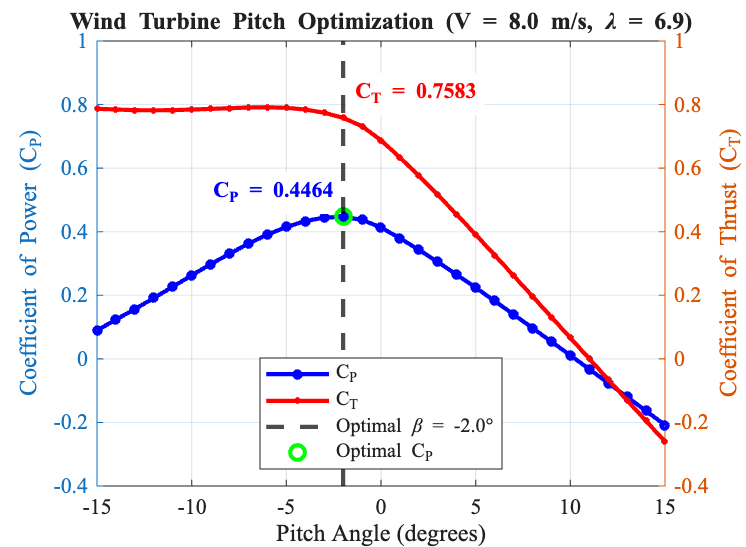
\includegraphics[width=0.5\textwidth]{media/Pitch_Optimization_Results.png}
  \caption{Coefficient of power and thrust as a function of pitch angle for wind speed of 8 m/s.}
  \label{fig:cp_ct_vs_pitch}
\end{figure}

The optimization revealed that the maximum coefficient of power occurs at a pitch angle of $\approx -2^{\circ}$, achieving $C_P = 0.4464$ with a corresponding thrust coefficient of $C_T = 0.7583$. This negative pitch angle is typical for lower wind speeds, as it increases the effective angle of attack and maximizes the lift-to-drag ratio, therefore optimizing power extraction.

The results demonstrate the importance of pitch control in wind turbine operation, as the pitch angle has significant effect on the available power output of the wind turbine. 

\subsubsection{Two-Dimensional Parameter Optimization}

A comprehensive two-dimensional optimization was performed to simultaneously optimize both pitch angle and tip speed ratio for a wind speed of 6 m/s. The analysis swept pitch angles from $-15^{\circ}$ to $+15^{\circ}$ and tip speed ratios from 8 to 13, as shown in Figure \ref{fig:cp_2d}.

\begin{figure}[H]
  \centering
  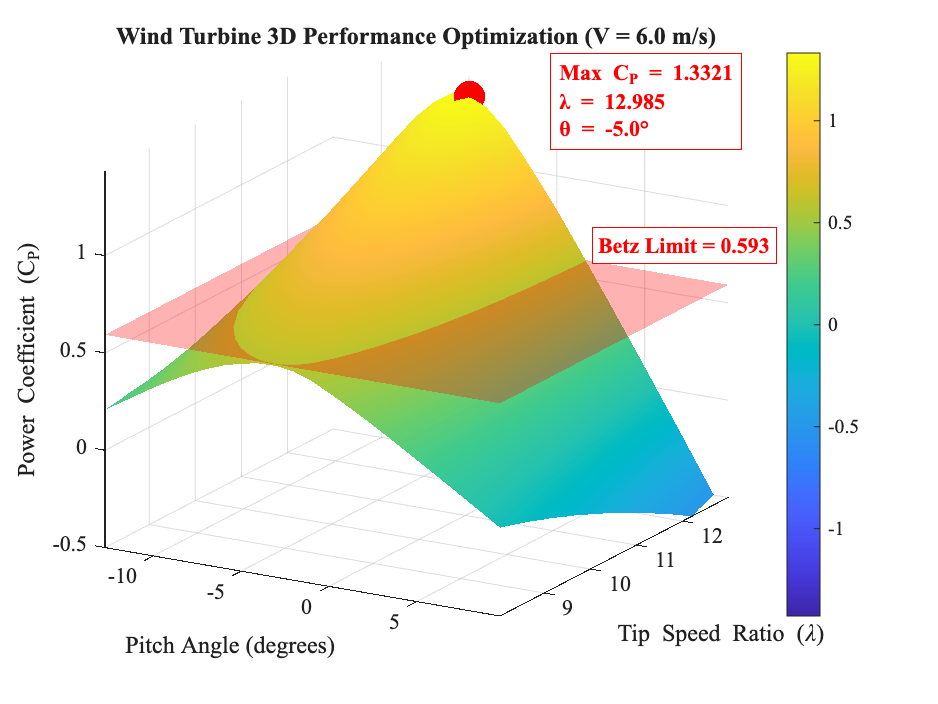
\includegraphics[width=0.6\textwidth]{media/2D_CP_Optimization_Results.png}
  \caption{Two-dimensional optimization results showing coefficient of power as a function of pitch angle and tip speed ratio for wind speed of 6 m/s.}
  \label{fig:cp_2d}
\end{figure}

The optimization identified an optimal operating point at a pitch angle of $\approx -5^{\circ}$ and tip speed ratio of $\approx 13$, yielding a coefficient of power of $C_P = 1.3321$. However, this result exceeds both the Betz limit (0.5926) and the theoretical maximum of 1.0, indicating a fundamental limitation of the model.

This unphysical result occurs because the BEM theory assumptions, specifically the tangential induction factor $a'$, break down under low wind speed and high tip speed ratio conditions. The model's inability to accurately predict performance in this regime highlights the importance of understanding model limitations and the need for more sophisticated analysis methods for extreme operating conditions.
\subsubsection{Power Limiting Analysis}

For higher wind speed conditions (14.6 m/s), the analysis determined the minimum pitch angle required to limit power output to the rated capacity of 2.5 MW. Figure \ref{fig:power_vs_pitch} shows the power output as a function of pitch angle, with the rated power limit indicated.

\begin{figure}[H]
  \centering
  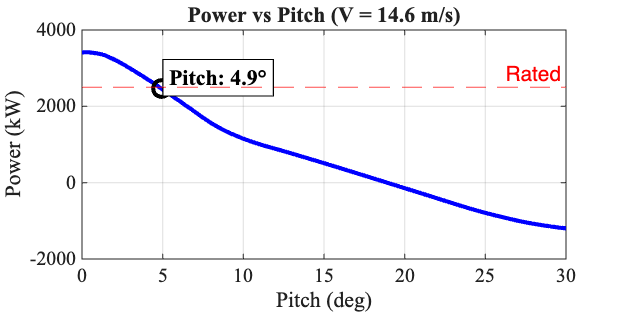
\includegraphics[width=0.5\textwidth]{media/Deliverable4_Power_vs_Pitch.png}
  \caption{Power vs. pitch angle at high wind speed with rated power line.}
  \label{fig:power_vs_pitch}
\end{figure}

The analysis revealed that a minimum pitch angle of $\approx 4.9^{\circ}$ is required to prevent power output from exceeding the rated capacity under these conditions.
This result demonstrates the critical importance of pitch control systems in wind turbine operation, particularly for maintaining safe operation under high wind conditions while maximizing energy capture at lower wind speeds. 

\subsection{Structural Analysis Results}

The structural analysis evaluated the tower's response to aerodynamic and gravitational loading through three key assessments: deflection analysis, static failure evaluation, and fatigue assessment.

\subsubsection{Tower Deflection Analysis}

The tower deflection analysis employed Euler-Bernoulli beam theory to model the structure as a cantilevered beam with variable cross-section. The analysis considered the distributed wind loading, which varies with height according to the atmospheric boundary layer profile, and the distributed nacelle thrust force.

The results showed a maximum tower deflection of $\approx 0.383$ meters, which represents $\approx 0.25\%$ of the total tower height. This deflection is well within acceptable limits for wind turbine tower design and occurs entirely within the elastic deformation range, ensuring no permanent damage to the structure.
\begin{figure}[H]
  \centering
  \begin{minipage}{0.49\textwidth}
    \centering
    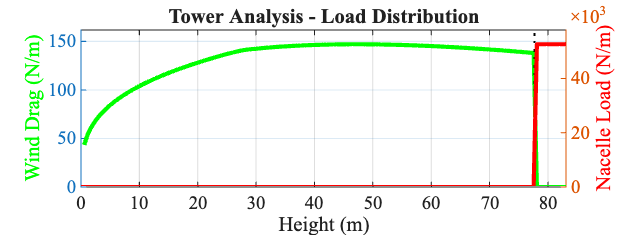
\includegraphics[width=\linewidth]{media/Tower_Load_Distribution.png}
    \captionof{figure}{Distributed wind drag and nacelle load along height for both load cases.}
    \label{fig:tower_load_distribution}
  \end{minipage}
  \hfill
  \begin{minipage}{0.49\textwidth}
    \centering
    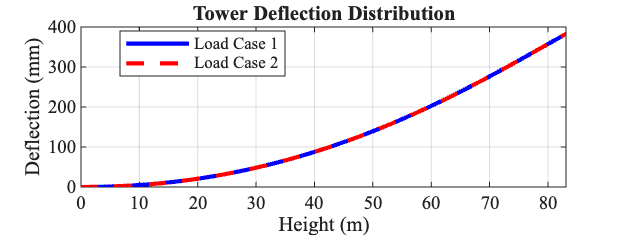
\includegraphics[width=\linewidth]{media/Tower_Deflection_Only.png}
    \captionof{figure}{Tower deflection under loading conditions, showing displacement along the height of the tower.}
    \label{fig:tower_deflection}
  \end{minipage}
\end{figure}


\subsubsection{Static Failure Analysis}

The static failure analysis evaluated the tower's structural integrity under maximum loading conditions using three established failure theories. The analysis focused on the maximum bending stress at the tower base, where the bending moment reaches its peak value as seen in Figure \ref{fig:tower_moment_distribution}.

\begin{figure}[h]
  \centering
  \begin{minipage}{0.49\textwidth}
    \centering
    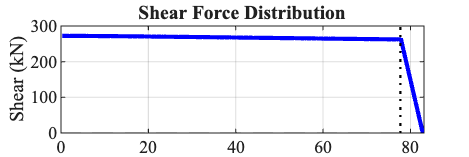
\includegraphics[width=\linewidth]{media/Shear_Distribution.png}
    \captionof{figure}{Shear force distribution.}
    \label{fig:tower_shear_distribution}
  \end{minipage}
  \hfill
  \begin{minipage}{0.49\textwidth}
    \centering
    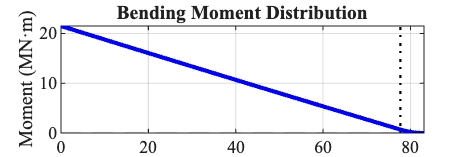
\includegraphics[width=\linewidth]{media/Bending_Moment_Distribution.png}
    \captionof{figure}{Bending moment distribution.}
    \label{fig:tower_moment_distribution}
  \end{minipage}
  \\
  \vspace{0.5em}
  \begin{minipage}{0.49\textwidth}
    \centering
    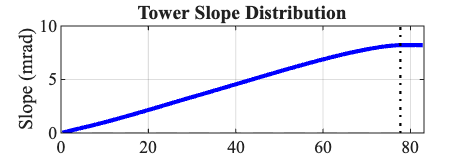
\includegraphics[width=\linewidth]{media/Slope_Distribution.png}
    \captionof{figure}{Slope distribution.}
    \label{fig:tower_slope_distribution}
  \end{minipage}
  \hfill
  \begin{minipage}{0.49\textwidth}
    \centering
    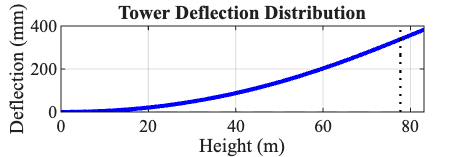
\includegraphics[width=\linewidth]{media/Tower_Deflection_Analysis.png}
    \captionof{figure}{Deflection distribution.}
    \label{fig:tower_deflection_distribution}
  \end{minipage}
\end{figure}


Using a yield strength of 345 MPa, the safety factors were calculated for all three failure theories:
\begin{itemize}
    \item Maximum Normal Stress Theory (Eq.~\ref{eq:mnst}): $n = 8.11$
    \item Maximum Shear Stress Theory (Eq.~\ref{eq:msst}): $n = 8.11$
    \item Distortion Energy Theory (Eq.~\ref{eq:det}): $n = 8.11$
\end{itemize}

All three theories yield identical safety factors of 8.11 due to the pure uniaxial bending simplification. This substantial safety margin exceeds the recommended minimum safety factor of 2.0 for wind turbine applications, confirming that the tower will not fail under static loading conditions. 
\subsubsection{Fatigue Analysis}

The fatigue analysis employed the modified Goodman criteria to assess the tower's long-term structural integrity under cyclic loading conditions. The analysis considered the alternating and mean stress components resulting from wind-induced loading variations.

The endurance limit was calculated from the ultimate tensile strength of 450 MPa using the appropriate modification factors, yielding an endurance limit of 148.75 MPa. The fatigue safety factor was then calculated using the modified Goodman equation, resulting in a safety factor of $n = 3.418$.

This safety factor significantly exceeds the recommended minimum of 2.0 for wind turbine applications, indicating that the tower can safely operate under the analyzed loading conditions without fatigue failure. The Goodman diagram (Figure \ref{fig:goodman}) provides a visual representation of the fatigue loading case, showing the relationship between mean and alternating stresses and the safe operating region.

\begin{figure}[H]
  \centering
  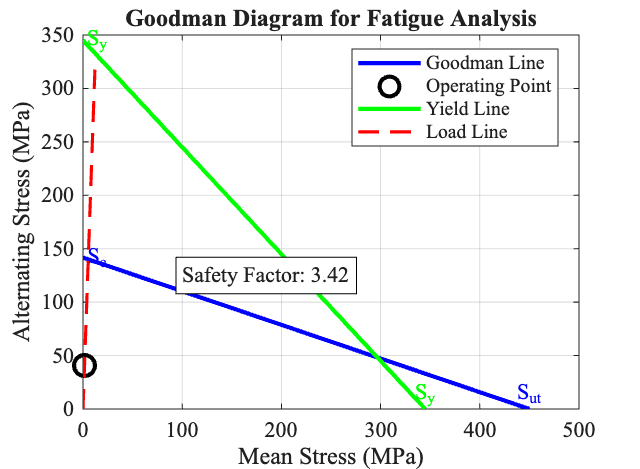
\includegraphics[width=0.5\textwidth]{media/Goodman_Diagram_Analysis.png}
  \caption{Goodman diagram showing fatigue loading case with mean and alternating stress components.}
  \label{fig:goodman}
\end{figure} 

\section{Conclusion}

This comprehensive analysis of the Clipper Liberty C96 wind turbine has successfully evaluated both the aerodynamic performance and structural integrity of the system under various operating conditions. The study employed established engineering methodologies including Blade Element Momentum theory for aerodynamic analysis and beam theory with multiple failure criteria for structural assessment.

The analysis successfully demonstrated that the Clipper Liberty C96 wind turbine operates safely and efficiently under the analyzed conditions. The aerodynamic performance is within expected ranges, and the structural integrity is well within safety margins.

\newpage
% References
\nocite{*}
\bibliographystyle{ieeetr}
\bibliography{references}

\end{document}
